\documentclass[a4paper,11pt]{article}
\usepackage[english]{babel}
\usepackage[T1]{fontenc}
\usepackage{fancyhdr}
\usepackage{graphicx}
\usepackage{a4wide}
\usepackage{numprint}
\usepackage{url}
\usepackage{cite}
\usepackage{multirow}
\usepackage{moreverb}
\usepackage{lastpage}
\usepackage{enumerate}
\pagestyle{fancy}

\author{Viktor Collin \\ <\url{vcollin@kth.se}> \\ 19880316-0277 \and Simon \"{O}sterman \\ <\url{simost@kth.se}> \\ 19880205-0156}
\title{\textbf{DH2323 Computer Graphics with Interaction \\ Lab 2 : Raytracer}}

\fancyhead[L]{\textbf{DH2323 : Lab 2} }
\fancyhead[R]{Viktor Collin \& Simon \"{O}sterman : Page \thepage }
\fancyfoot{}{}

\begin{document}
\maketitle
\begin{center}
Total pages: \pageref{LastPage}
\end{center}
\thispagestyle{empty}

\clearpage
\setcounter{page}{1}
\section{Introduction}
The purpose of this lab is to learn how to build a raytracer and use it to render an image of a 3D environment that consists of triangular shapes. The lab also includes light models, shading and camera movement. 
\section{Assignment}
The assignment is to implement a raytracer which can create images given a 3D-model by tracing the rays reaching a simulated camera. The implementation should be done in several steps, each with new functionality or other improvements. The final implementation should include a mobile camera, simulated light-sources as well as light reflection for diffuse surfaces.
\section{Method}
\subsection{First implementation}
As a first step we built our raytracer to send a ray thru each pixel on the screen and fining the closes intersection with the predefined model of the room, then it render that pixel to be the color of the intersected shape. If the ray did not hit any shape we  render the pixel to be black. See the output of this in figure \ref{fig1}.

\subsection{Camera movement}
Next step was to implement an interactive environment were the user with the help of the keyboard should be able to move and rotate the camera. Rotations is implemented by increasing or decreasing an angle and then updating the rotation matrix \verb|R|. movement in the forward and backward directions is then done by multiplying \verb|R| with a movement speed in the \verb|z| direction. The rays sent thru each pixel is then sent in the direction the camera is facing.

\subsection{Direct light}
To introduce shading we introduced a light source in the ceiling of the room. When the ray from the camera hit a shape we sent a new ray from the intersection point towards the light source to see if there was an object shadowing that pixel. If so the pixel was painted black otherwise the amount of light was calculated based on the distance from the light. At first this implementation did not take in to consideration the color of the shape that was hit by the first ray. See the output of this in figure \ref{fig2}.  
\section{Result}

\begin{figure}[h!]
	\centering
	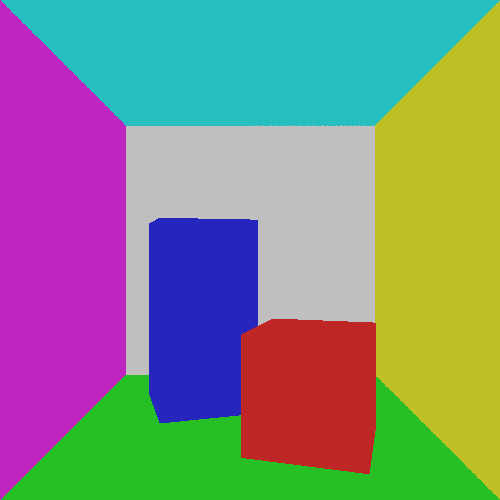
\includegraphics[width=0.75\linewidth]{screenshot1.png}
	\caption{Output from first run}
	\label{fig1}
\end{figure}

\begin{figure}[h!]
	\centering
	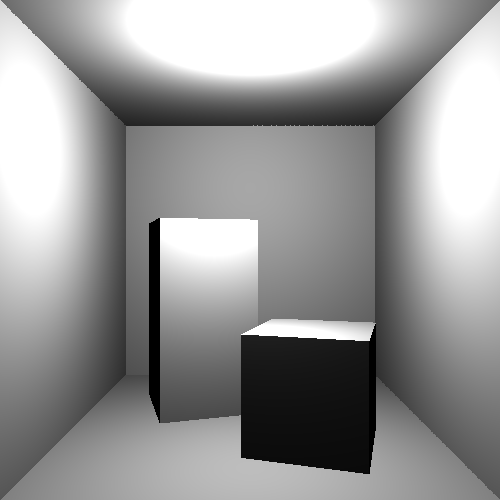
\includegraphics[width=0.75\linewidth]{screenshot2.png}
	\caption{Output from the direct light model}
	\label{fig2}
\end{figure}

\end{document}
